
\chapter{プログラムの制作過程と解説}
この章では今回作成したプログラムのうち,波の干渉と回折現象を視覚化したプログラムの制作過程の記述と処理の解説を行う.
\section{Processing言語}
本研究のプログラムに使用した言語はProcessing言語である.
Processing言語は以下に挙げるような特徴を有している\cite{ishikawa}.
\begin{enumerate}
\item 基本文法はJavaをベースに記法を簡単化したものであり,
インタラクティブソフトウェアやビジュアルプレゼンテーションを容易に実現することに特化している.
%\item 環境構築が非常に容易かつ無償で行える.これはgithubプラットフォームでの共同開発を試みていた榊さんの利点
\item Windows, iOS, Androidのタブレット端末で用いられる3つのプラットフォーム全てで動作する. %//なんで動作するかを調べる
\end{enumerate}
1の特徴からは,視覚化プログラムの作成に適していると言える.  2の特徴からは,学習者があらゆるタブレット端末を使用してもプログラムが動作することが言える.これらの理由から,本研究で使用するプログラミング言語に最も適していると考えた.

\section{波の干渉の描写}
回折,反射,屈折の性質を可視化するためには多数の波を生成し,それらに重ね合わせの原理を適用しなければならない.そこで複数の点源から波を生成した上で,重ね合わせの原理によって生じる干渉を視覚化するプログラムを作成した.

\subsection{波源から波の代わりとなる円を描写するプログラム}
最初は波の干渉の描写を実現するために,図\ref{fig:missdraw}のように,画面左上から右下へ進行する斜めの線を入射波に見立て,入射波が波源として設定した座標を通過すると,波源から波の代わりとなる円を描写するプログラムを作成した.この後,円が重なった部分の色を変化させたり複数の円の包絡線を太く描写することを考えた. しかし計算アルゴリズムが非常に複雑になることや,処理速度が追いつかないことからこの方法は断念した.

\begin{figure}[H]
 \begin{center}
  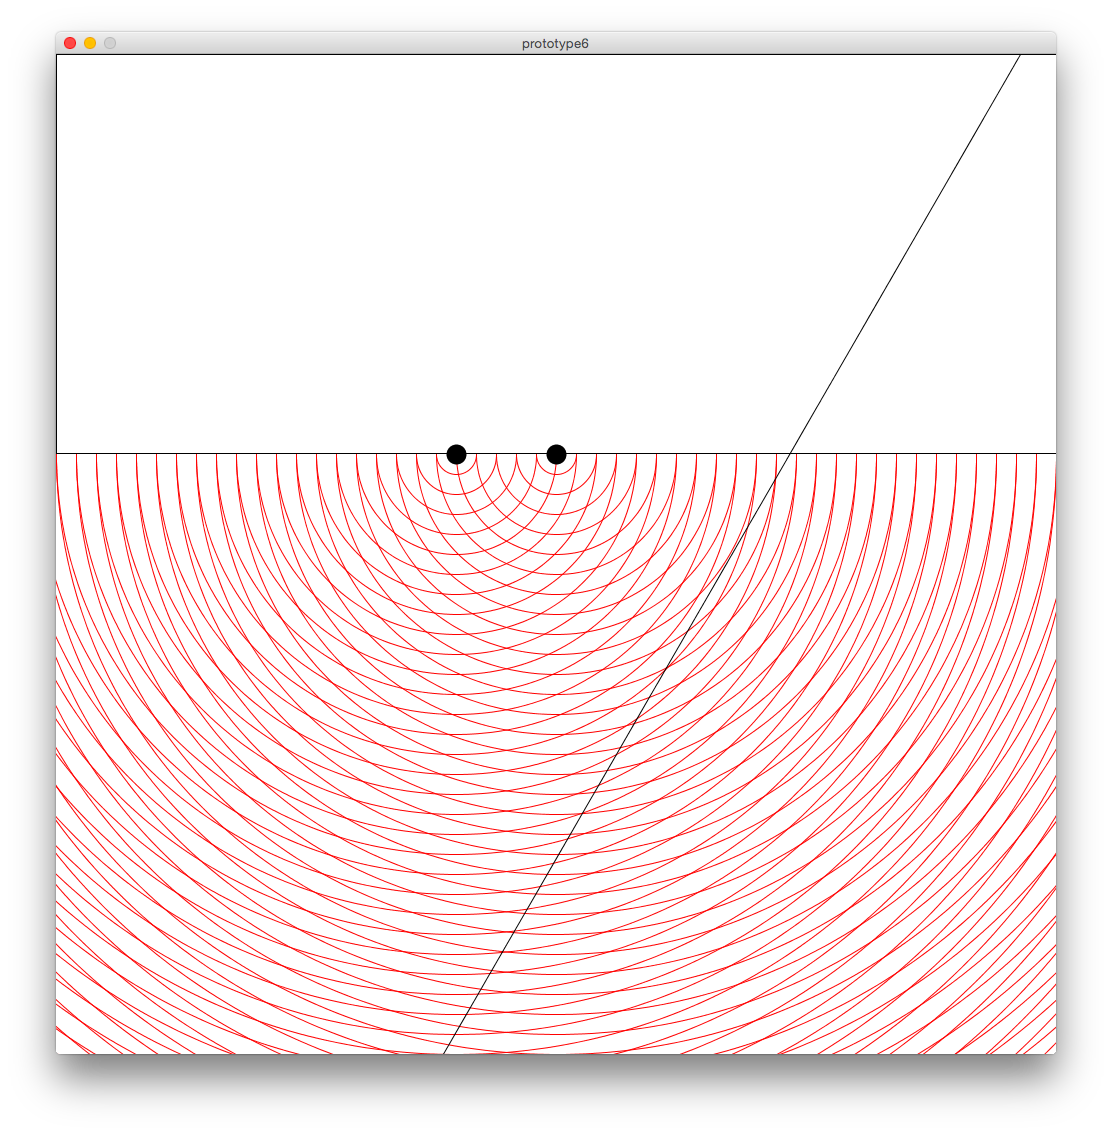
\includegraphics[width=70mm]{../implement/miss_draw.png}
 \end{center}
 \caption{プログラムの動作画面.}
 \label{fig:missdraw}
\end{figure}
そこで各ピクセルが波源からの距離,波源の生成された時間,波源から生成される波の波長と周期を基にして自らの地点の位相を計算する手法を考案した.

\subsection{平面波描写のアルゴリズム} 
\label{sec:algo}
アルゴリズムは以下の手順である.
\begin{enumerate}
 \item 平面波の変位計算を何ピクセルごとに行うかを指定する.これにより描写領域のピクセル数を擬似的に変更する.これ以降,説明のために擬似的に変更したピクセルの単位を\emph{擬似ピクセル}と記す.
  \item 描写領域がクリックされると波源の座標情報が追加される.この際1つの波源ごとに,各擬似ピクセルとの距離を計算し,各擬似ピクセルに対応した配列(point\_distance[i][j])に格納している.
  \item 点源とは異なる座標の点における変位の計算を,全ての点源と全ての擬似ピクセルに対しおこない,これによって得られた変位の値を,それぞれの擬似ピクセル上での変位に変換し,各擬似ピクセルごとに設けた配列(point\_[i][j])に足し合わせていく.
  \item 各擬似ピクセルごとの変位の値を基にして,値に応じた色の点を描写する.
 \item 描画領域がクリックされた瞬間のみ手順2を,そうでなければ手順3-4を毎フレームごとに繰り返して平面波の挙動を継続的に描写し続ける.
 \end{enumerate}
 なお,手順2の段階で配列(point\_distance[i][j])に値を格納しているのは,手順3での異なる座標の点における変位の計算をおこなう際,点源と擬似ピクセルの距離が必要であるため,あらかじめ計算させることで処理を軽くするためである.

\subsection{描画領域のピクセル数を擬似的に変更する方法}
\ref{sec:algo}に描写領域のピクセル数を擬似的に変更するとあるが,これを行う事により平面波描写の処理を大幅に軽減することができる.

まず,図\ref{fig:pxcelone}のように8×8ピクセルの描写領域があるとする.
これに対し\ref{sec:algo}のアルゴリズムを適用すると,フレームごとに8×8の64個の座標それぞれに対し変位計算を行うことになる.
一方,図\ref{fig:pxceltwo}のように8×8の描写領域に対し,変位計算を2ピクセルごとに行うとするならば,フレームごとの位相計算は4×4の16個の座標に対してすればよい.つまり計算回数は図\ref{fig:pxcelone}の時と比べ,4分の1回となる.

今回作成したプログラムは描写領域を400×400ピクセルとしているため,
ピクセル数を変更しなければフレームごとに160000回の変位計算を行うことになるが,
4ピクセルごとに変位計算を行うことで計算回数を10000回まで削減した.

\begin{figure}[H]
 \begin{center}
  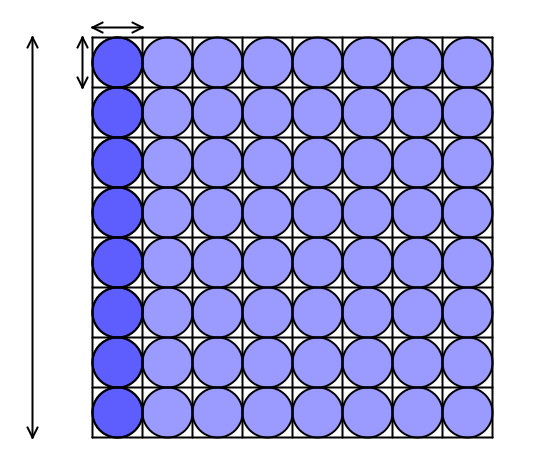
\includegraphics[width=90mm]{../implement/1pxcel.png}
 \end{center}
 \caption{8$×$8の描写領域に色を塗る場合.}
 \label{fig:pxcelone}
\end{figure}


\begin{figure}[H]
 \begin{center}
  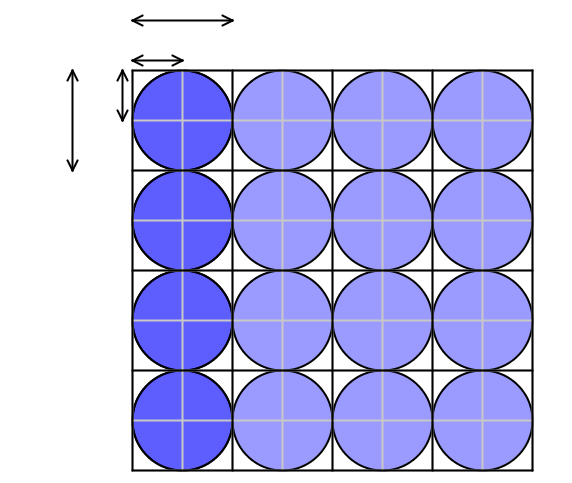
\includegraphics[width=90mm]{../implement/2pxcel.png}
 \end{center}
 \caption{8$×$8の描写領域を擬似的に4$×$4に変更する場合.}
 \label{fig:pxceltwo}
\end{figure}


\newpage
またプログラムの擬似ピクセル数はグローバル変数のpoint\_regulationの値を変えることで変更可能である.
図\ref{fig:1pxceldraw}は擬似ピクセル数を1(変更なし)にした時の波の描写,
 図\ref{fig:8pxceldraw}は擬似ピクセル数を8にした時の波の描写である.
 
 なお,図\ref{fig:1pxceldraw},図\ref{fig:8pxceldraw}以外で論文に用いているプログラムの動作画面は全て擬似ピクセル数を4で設定したものである.


\begin{figure}[H]
 \begin{center}
  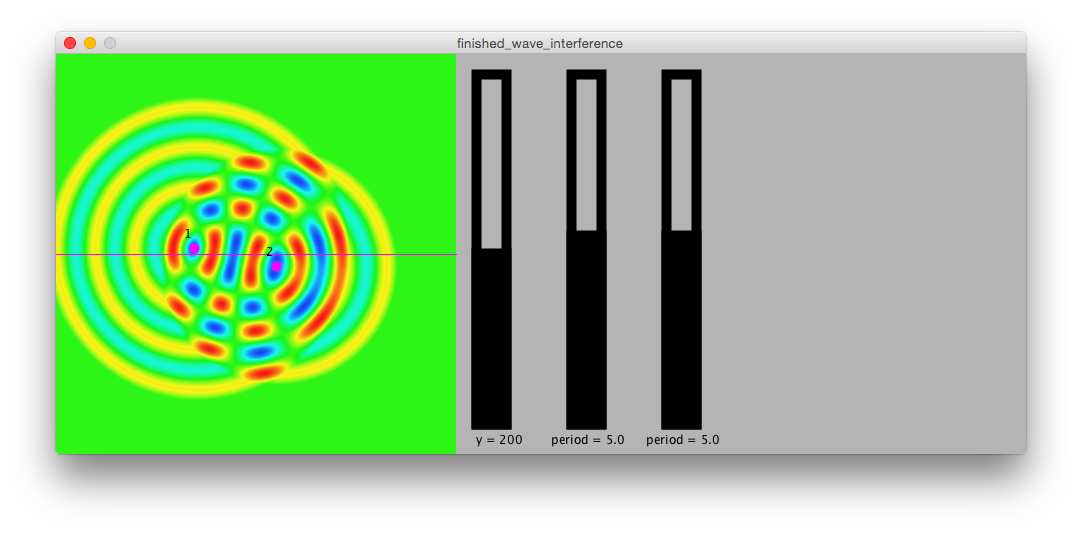
\includegraphics[width=140mm]{../implement/pointregulation1.png}
 \end{center}
 \caption{擬似ピクセル数を1に設定した時の波の描写.}
 \label{fig:1pxceldraw}
\end{figure}

\begin{figure}[H]
 \begin{center}
  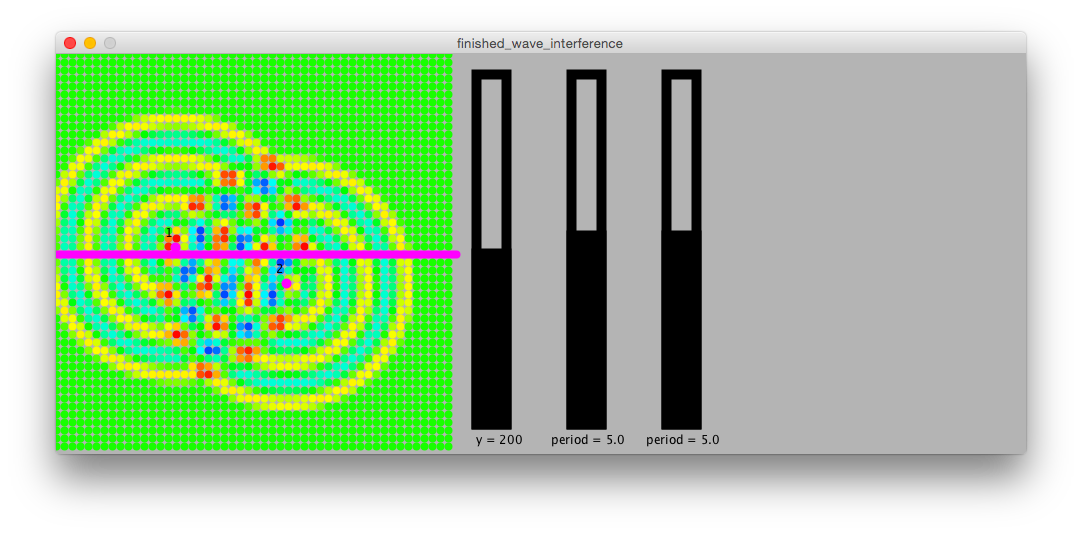
\includegraphics[width=140mm]{../implement/pointregulation8.png}
 \end{center}
 \caption{画面の画素数を8に設定した時の波の描写.}
 \label{fig:8pxceldraw}
\end{figure}


\subsection{波の色の表現方法}

Processing言語では色を表現する際,RGBカラーモデルとHSBカラーモデルの2つを用途に応じて使用することができる.
RGBカラーモデルは赤(Red),緑(Green),青(Blue)の3つの色を様々な配分で混ぜ合わせることで色を表現し,
HSBカラーモデルは色相(Hue),彩度(Saturation),明度(Brightness)の組み合わせによって色を表現する.

図\ref{fig:hsb}はHSBモードでS(彩度)=100,B(明度)=100に設定し,H(色相)を変更した際の色の変化である.図の右側の数字はH(色相)の値を示している.
このようにHSBカラーモデルではRGBカラーモデルとは異なり,赤,緑,青の3色を1つの値(色相)を入れ替えるだけで表現できる特徴があるため,プログラムではこのモデルを採用した.
\begin{figure}[H]
 \begin{center}
  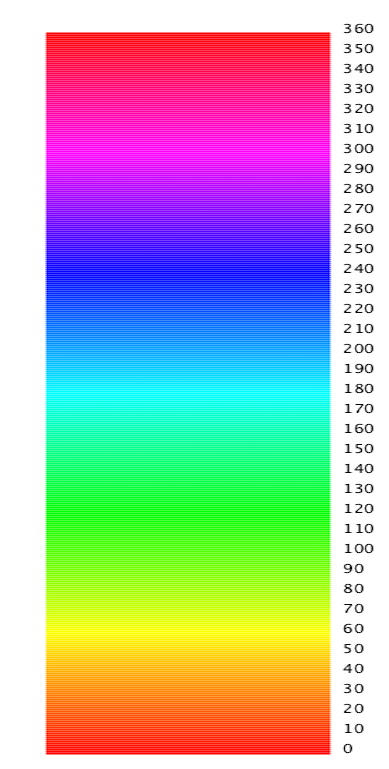
\includegraphics[width=40mm]{../implement/hsb.png}
 \end{center}
 \caption{HSBモードで色相の値を上下させた時の色の変化.}
 \label{fig:hsb}
\end{figure}


プログラムでは,擬似ピクセルごとに記録された波の変位に応じて描画する点の色を変更する.
この時,波の変位が高い時は赤色,変位が0に近い場合は緑色,変位が低い場合には青色で描写するように処理を行う.
\begin{framed}
{\small
\begin{verbatim}
point[i][j] += number_wave_point;
stroke( (number_wave_point2- point[i][j])*(230/number_wave_point2),100,100);
\end{verbatim}}
\end{framed}
この処理は各擬似ピクセルごとの(変位)を0$\sim$230までの値に変換するものである.

まず(point[i][j])に格納されている擬似ピクセルの変位に現在の波源の数を足す.
例えば点源が3つある場合,各擬似ピクセルの変位は波源の振幅が1であるため-3$\sim$3までの値をとる.ここに点源の数を足すと(point[i][j])の値は0$\sim$6までの値をとり,全て正の数となる.
次に変位の値が大きいほど赤色に近づけるようにするため,点源の数の2倍(number\_wave\_point2)から(point[i][j])を減算する.
最後に点源の数の2倍で割ることで値を0$\sim$1の範囲にしてから230を掛けることで,変位の変化と色の変化を連動させることができる.

\section{Elementary\_wavesクラス} 
このクラスは波源と,波源から生じる波に関する処理を行っている.
 \begin{framed}
{\small
\begin{verbatim}
class Elementary_waves{
  float center_x; float center_y;
  float lambda;
  float period;
  float created_time;
  float period_max; float period_min;
  float lambda_max; float lambda_min;

  Elementary_waves(float _center_x, float _center_y, 
  float _lambda, float _period, 
    float _period_min, float _period_max, 
    float _lambda_min, float _lambda_max){
    	center_x = _center_x; center_y = _center_y;
    	lambda = _lambda;
    	period = _period;
    	period_max = _period_max; period_min = _period_min;
    	lambda_max = _lambda_max; lambda_min = _lambda_min;
    	created_time = 0; 
    }
    float now_displacement_y(float distance, float lambda, 
    float period, float time_adjustment){
    float time_phase_adjustment;
    time_phase_adjustment = 
    ((millis()-time_adjustment)/1000.0)*(360.0 / period); 
    float distance_lambda_adjustment = 
    (distance%lambda)/lambda*(360.0);
    float y = 
    sin(radians(time_phase_adjustment - 
    distance_lambda_adjustment));
    return y;
  }
}
}
\end{verbatim}}
\end{framed}
 
 
 \subsection{メンバ変数}
 クラスElementary\_wavesは波源が持つ様々なパラメータをメンバ変数としている.メンバ変数を以下に示す.
 \begin{description}
 \item[center\_x, center\_y]\mbox{}\\
 波源のx座標,y座標を記録する.
 \item[lambda]\mbox{}\\
 波源から生じる波の波長を記録する.
  \item[period]\mbox{}\\
  波源から生じる波の波長を記録する.
   \item[period\_max, period\_min]\mbox{}\\
   スライダーで周期を調節する際の最大値,最小値を記録する.
    \item[lambda\_max,lambda\_min]\mbox{}\\
    スライダーで波長を調節する際の最大値,最小値を記録する.
     \item[created\_time]\mbox{}\\
     波源が生成された時間を記録する.
 \end{description}

プログラムではクラス配列としてクラスElementary\_wavesのインスタンスを複数生成し,各波源としている.


\subsection{点源とは異なる座標の点における変位の計算の実装}
\ref{sec:calculatey}の方法で任意の擬似ピクセル上の変位計算を行うためのメンバ関数,now\_displacement\_yを実装した.

引数のdistanceにはある波源と,ある擬似ピクセルとの距離を代入する.
lambdaにはある波源から生成される波の波長,periodにはある波源から生成される波の周期を代入する.
time\_adjustmentにはある波源が生成された際に,プログラムを起動してから経過していた時間を代入する.

Processing言語にはプログラムが起動してからのミリ秒(1/1000秒)の数を返り値とするmillis()という関数が備えられている.計算上ミリ秒ではなく秒数に直した方が都合がいいので,millisの値を1000で割っている.

またsin関数の中の値をradians()関数によって角度の単位を「度」からラジアンに変換している.Processing言語のパラメータの単位はラジアンなのでこのような処理を施している.

\section{指定したy座標におけるx座標の変位の描写}
\ref{sec:check}節で説明した,y軸上の変位を描写するアルゴリズムを以下に示す.
\begin{enumerate}
\item 各擬似ピクセルの変位を計算する.
\item 手順1によって得られた値を擬似ピクセルごとに設けられた配列に減算して格納する.
\item drawモードで赤線が描写されている座標の変位を取得し,振幅となる値を掛けた上で点として描写する.
\item 変位を測る目盛りを描写する.
\item 1-4を繰り返す.
\end{enumerate}
手順2で減算する理由は,Processing言語で用いられる座標系を,数学等で用いられる一般的な座標系に変換して描写するためである.

\section{Sliderクラス}
波の干渉の視覚化プログラム内で,榊の作成したプログラムを元に,波源の数をいくら増やした場合でもスライダーの数がそれに応じて増えるようにクラス化した\cite{sakaki}.コードを以下に記す.
\begin{framed}
{\small
\begin{verbatim}
class Sliders{
  int position_x; int position_y;
  int slider_height; int slider_width;
  int digit;
  int number_tickmarks;
  int num_separator;
  float min; float max;
  float cordinate_y;
  String variable_name;
  boolean draw_flag;
  boolean slider_dragged;

  Sliders(int _position_x, int _position_y, int _slider_height,
   int _slider_width, float _min, float _max,
    int _number_tickmarks,int _digit, String _variable_name){
    position_x = _position_x; position_y = _position_y;
    slider_height = _slider_height; slider_width = _slider_width;
    min = _min; max = _max;
    number_tickmarks = _number_tickmarks;
    digit = _digit;
    variable_name = _variable_name;
    draw_flag = false;
    slider_dragged = false;
  }

  float draw_slider(float variable_value){
    if(draw_flag == true){
      num_separator =
       (int)map(variable_value, min, max, number_tickmarks-1,0); 
      cordinate_y = 
      position_y + slider_height - 
      ((float)slider_height / (number_tickmarks-1))*num_separator; 
      fill(255);
      noStroke();                                                       
      rect(position_x, position_y + slider_height, slider_width+50, 30); 
      stroke(1);
      rect(position_x, position_y, slider_width, slider_height);
      fill(0);
      rect(position_x, cordinate_y, slider_width, 
      position_y + slider_height - cordinate_y);
      if(variable_name == "y = "){text(variable_name +
      nf(variable_value*point_regulation,1,digit),
       position_x, position_y + slider_height + 20);
      }else{
        text(variable_name + nf(variable_value,1,digit),
         position_x-20, position_y + slider_height + 20);
      }
      if(mousePressed==false) slider_dragged=false;
      if(mouseX >= position_x & mouseX <= position_x + slider_width 
      & mouseY<=cordinate_y+10 & mouseY>= cordinate_y-10){
        if(mousePressed){
          slider_dragged= true;
        }
      }

if(slider_dragged){
        num_separator+= 
        (int)((cordinate_y - mouseY)/
        ((float)slider_height /(number_tickmarks-1))); 
        num_separator = 
        constrain(num_separator, 0, number_tickmarks-1); 
        if(digit == 0){
          variable_value = 
          (max-min) - round(map(num_separator, 0, 
          number_tickmarks-1, min, max)); 
        }else{
          variable_value = 
          (max+min) - 
          map(num_separator, 0, number_tickmarks-1, min, max);
        }
        return variable_value;
      }else{
        return variable_value;
      }
    }else{
      return variable_value;
    }
  }
}
\end{verbatim}}
\end{framed}

このプログラムを利用する準備として,擬似ピクセル数を格納する変数point\_regulationをグローバル変数で定義しておく必要がある.

 \subsection{メンバ変数}
 クラスSliders内の変数を以下に示す.
 \begin{description}
 \item[position\_x, potision\_y]\mbox{}\\
 スライダー左上のx座標,y座標を記録する.
 \item[slider\_height,slider\_width]\mbox{}\\
 縦横の幅を記録する.
  \item[digit]\mbox{}\\
  返り値の桁数を記録する.
   \item[min,max]\mbox{}\\
   値の最小値,最大値を記録する.
    \item[number\_tickmarks]\mbox{}\\
    返す値を何段階で調節できるようにするかを記録する.
    例えばmin=0,max=10の時,number\_tickmarksを11に設定すると0,1,2...9.10の11段階で値を調節できるスライダーとなる.
    \item[num\_separator]\mbox{}\\
    調節する変数の値がスライダーの何段階目の値に位置しているかを記録する.
        \item[cordinate\_y]\mbox{}\\
        調節している変数の値に応じたy座標を記録する.
     \item[variable\_name]\mbox{}\\
     スライダー下部に表示される,調節する変数名の文字列を記録する.
          \item[draw\_flag]\mbox{}\\
     スライダーを画面に表示するかどうかの判定で利用する.
          \item[slider\_dragged]\mbox{}\\
     スライダーの掴み判定の判定で利用する.
      \item[variable\_value(draw\_sliderの引数)]\mbox{}\\
      調節したい変数を格納している.
 \end{description}
 
  \subsection{処理の流れ}
\begin{enumerate}

\item 調整する変数の値から,その値が下から何段階目に位置するかを計算する
\item 段階の番号から,スライダー部分のy座標を計算する.
\item スライダーを描画する.
\item スライダーの掴み判定(slider\_drugged)を行う.
\item 掴み判定がtrueの場合,
\begin{enumerate}
\item マウスの移動距離に対応した段階数に値を加える.
\item 段階数から調節する変数の値を変更し,その値を返す.
\end{enumerate}
掴み判定がfalseの場合,
\begin{enumerate}
\item 調節する変数の値を変更せずにそのまま返す.
\end{enumerate}
\end{enumerate}

\section{回折現象の視覚化}
波の干渉プログラムで作成した平面波の描写をベースとして作成した.
波源のx座標の間隔は,障害物の間隔に関わらず10ピクセルとしている.実際の物理現象を考えると波源は無限に存在するので波源同士の間隔は存在しないと言えるが,仮に有限であったとしたら波源同士に間隔の差はないと考えたからである.















